%%%%%%%%%%%%%%%%%%%%%%%%%%%%%%%%%%%%%%%%%
% Thin Sectioned Essay
% LaTeX Template
% Version 1.0 (3/8/13)
%
% This template has downloaded from:
% http://www.LaTeXTemplates.com
%
% Original Author:
% Nicolas Diaz (nsdiaz@uc.cl) with extensive modifications by:
% Vel (vel@latextemplates.com)
%
% License:
% CC BY-NC-SA 3.0 (http://creativecommons.org/licenses/by-nc-sa/3.0/)
%
%%%%%%%%%%%%%%%%%%%%%%%%%%%%%%%%%%%%%%%%%

%----------------------------------------------------------------------------------------
%	PACKAGES AND OTHER DOCUMENT CONFIGURATIONS
%----------------------------------------------------------------------------------------

\documentclass[a4paper, 11pt]{article} % Font size (can be 10pt, 11pt or 12pt) and paper size (remove a4paper for US letter paper)

\usepackage[protrusion=true,expansion=true]{microtype} % Better typography
\usepackage{graphicx} % Required for including pictures
\usepackage{float}
\usepackage{wrapfig} % Allows in-line images
\usepackage{amsmath}
\usepackage{algorithm}
\usepackage[noend]{algpseudocode}
\usepackage{pifont}
\usepackage{lipsum}
\usepackage[nottoc,numbib]{tocbibind}

\makeatletter
\def\BState{\State\hskip-\ALG@thistlm}
\makeatother
\usepackage{subcaption}
\captionsetup{compatibility=false}
\usepackage{adjustbox}

\usepackage{mathpazo} % Use the Palatino font
\usepackage[T1]{fontenc} % Required for accented characters
\linespread{1.05} % Change line spacing here, Palatino benefits from a slight increase by default
zz
\makeatletter
\renewcommand\@biblabel[1]{\textbf{#1.}} % Change the square brackets for each bibliography item from '[1]' to '1.'
\renewcommand{\@listI}{\itemsep=0pt} % Reduce the space between items in the itemize environments and the bibliography

\renewcommand{\maketitle}{ % Customize the title - do not edit title and author name here, see the TITLE block below
\begin{flushright} % Right align
{\LARGE\@title} % Increase the font size of the title

\vspace{50pt} % Some vertical space between the title and author name

{\large\@author} % Author name
\\\@date % Date

\vspace{40pt} % Some vertical space between the author block and abstract
\end{flushright}
}

%----------------------------------------------------------------------------------------
%	TITLE
%----------------------------------------------------------------------------------------

\title{\textbf{TNM034 ABOB}}

% Author
\author{{Niklas Andersson, nikan278}, 
\\{Joakim Deborg, joade361}
\\{Gabriel Baravdish, gabba873}
\\{Lars Bergman, larbe444}} % Institution

\date{\today} % Date

%----------------------------------------------------------------------------------------

\begin{document}

\maketitle % Print the title section

%----------------------------------------------------------------------------------------
%	ABSTRACT AND KEYWORDS
%----------------------------------------------------------------------------------------

%\renewcommand{\abstractname}{Summary} % Uncomment to change the name of the abstract to something else

\begin{abstract}
This is abstract!
%Abstract
Face recognition has various fields and many applications... 

\end{abstract}

\vspace{30pt} % Some vertical space between the abstract and first section

%----------------------------------------------------------------------------------------
%	ESSAY BODY
%----------------------------------------------------------------------------------------

\newpage

\tableofcontents

\newpage

\section{Introduction}
\subsection{Aim}
The aim of this project work is to implement an algorithm in \textit{Matlab} that can detect and recognize human faces in different color images. The implementation should from an input image of an unknown face detect where in the image the face is located and make a decision if it belongs to a known person in the given database. Furthermore should the algorithm be tolerant for small rotations, translations and scaling inside the image plane as well as for varying tone values, lightning conditions, facial poses, background environments and degrees of blur. Other prerequisites for the project work were that the input image always include a front-faced portrait and that the images could be of varying size.


\subsection{Pipeline}
The pipeline of a standard frontal face authentication algorithm involves solving multiple sub problems such as \textit{preprocessing}, \textit{face detection} and \textit{face recognition}. Each of these sub problems can be solved in various ways and below we list our solutions.

\begin{itemize}
  \item \textbf{In the preprocessing phase} we use simple methods of color correction, namely black and white balancing. 
  \item \textbf{The face detection phase} is built around finding regions of skin in the \textit{YCbCr} color space and the combination of those regions with masks gathered through various segmentation steps. 
  \item \textbf{For the face recognition part} we base our algorithm upon on the \textit{Local Phase Quantization} (LPQ) algorithm. 

  % \emph{LPQ}\footnote{LPQ - Local phase quantization} and \emph{Eigenfaces} are described.
\end{itemize}


\section{Background}
%Background
\lipsum[10]

\section{Method}
%Method
\lipsum[10]

\section{Result}

\subsection{Face detection}


\begin{figure}[H]
\centering

\begin{subfigure}{0.65\textwidth}
\begin{subfigure}{.33\textwidth}
  \centering
  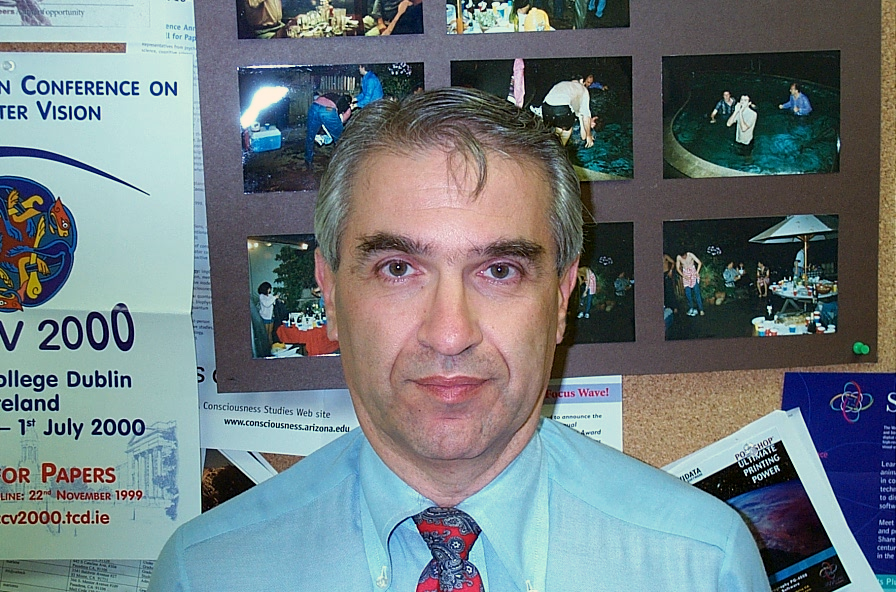
\includegraphics[width=0.95\textwidth]{img/fdResult1/input63.png}
  \caption{}
\end{subfigure}%
\begin{subfigure}{.33\textwidth}
  \centering
  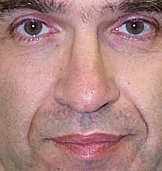
\includegraphics[width=0.6\textwidth]{img/fdResult1/output63.png}
  \caption{}
\end{subfigure}%
\end{subfigure}%
\begin{subfigure}{0.65\textwidth}
\begin{subfigure}{.33\textwidth}
  \centering
  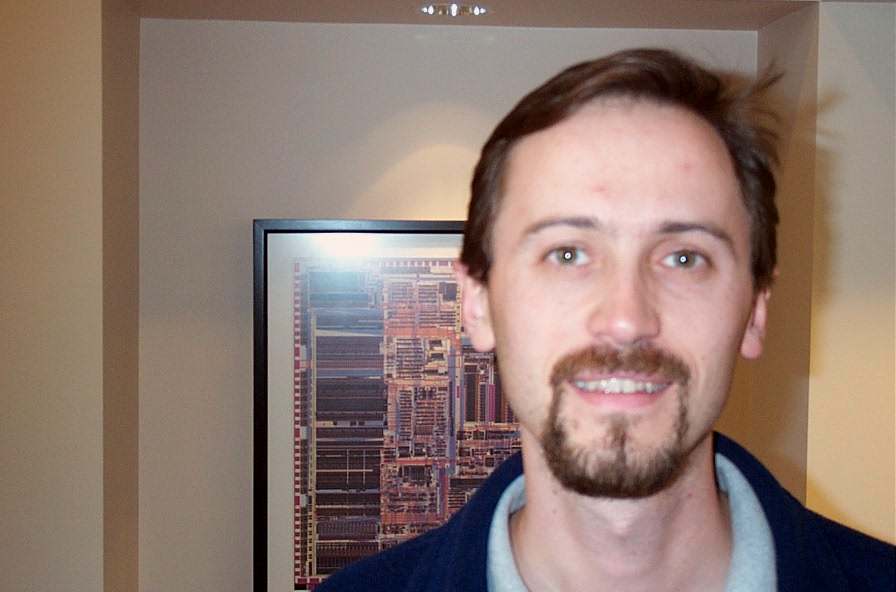
\includegraphics[width=0.95\textwidth]{img/fdResult1/input18.png}
  \caption{}
\end{subfigure}%
\begin{subfigure}{.33\textwidth}
  \centering
  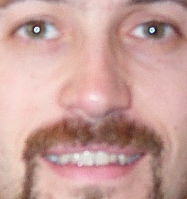
\includegraphics[width=0.6\textwidth]{img/fdResult1/output18.png}
  \caption{}
\end{subfigure}%
\end{subfigure}%

\begin{subfigure}{0.65\textwidth}
\begin{subfigure}{.33\textwidth}
  \centering
  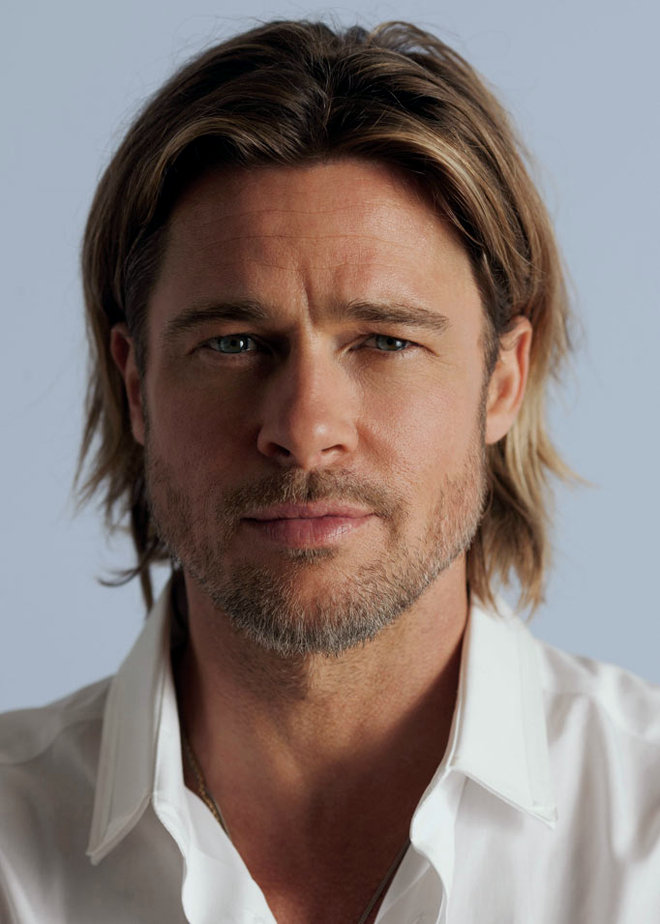
\includegraphics[width=0.95\textwidth]{img/fdResult2/input12.png}
  \caption{}
\end{subfigure}%
\begin{subfigure}{.33\textwidth}
  \centering
  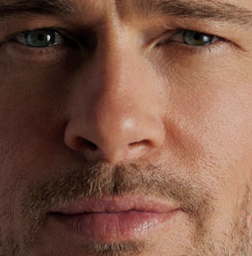
\includegraphics[width=0.6\textwidth]{img/fdResult2/output12.png}
  \caption{}
\end{subfigure}%
\end{subfigure}%
\begin{subfigure}{0.65\textwidth}
\begin{subfigure}{.33\textwidth}
  \centering
  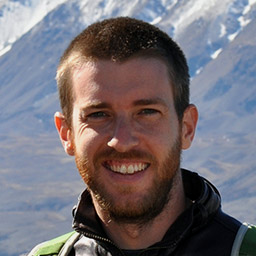
\includegraphics[width=0.95\textwidth]{img/fdResult2/input92.png}
  \caption{}
\end{subfigure}%
\begin{subfigure}{.33\textwidth}
  \centering
  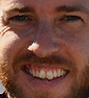
\includegraphics[width=0.6\textwidth]{img/fdResult2/output92.png}
  \caption{}
\end{subfigure}%
\end{subfigure}%

\begin{subfigure}{0.65\textwidth}
\begin{subfigure}{.33\textwidth}
  \centering
  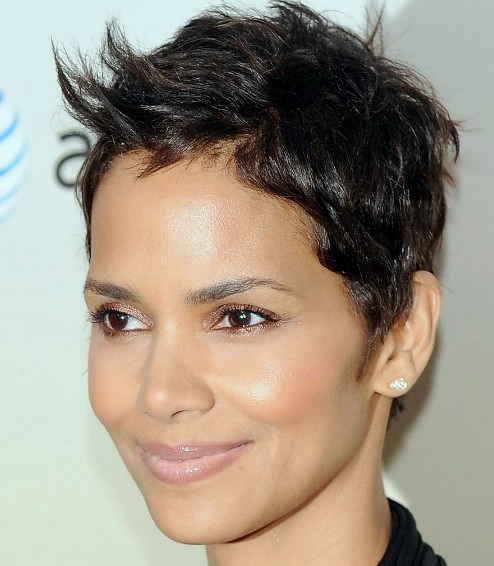
\includegraphics[width=0.95\textwidth]{img/fdResult2/input63.png}
  \caption{}
\end{subfigure}%
\begin{subfigure}{.33\textwidth}
  \centering
  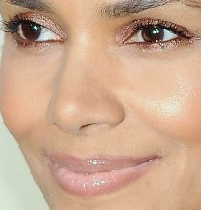
\includegraphics[width=0.6\textwidth]{img/fdResult2/output63.png}
  \caption{}
\end{subfigure}%
\end{subfigure}%
\begin{subfigure}{0.65\textwidth}
\begin{subfigure}{.33\textwidth}
  \centering
  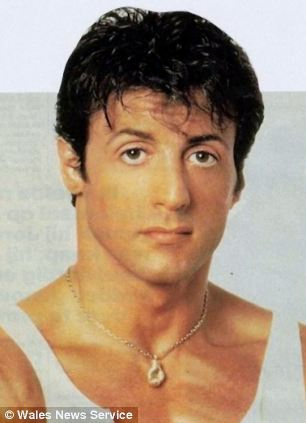
\includegraphics[width=0.95\textwidth]{img/fdResult2/input82.png}
  \caption{}
\end{subfigure}%
\begin{subfigure}{.33\textwidth}
  \centering
  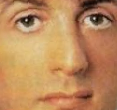
\includegraphics[width=0.6\textwidth]{img/fdResult2/output82.png}
  \caption{}
\end{subfigure}%
\end{subfigure}%

\begin{subfigure}{0.65\textwidth}
\begin{subfigure}{.33\textwidth}
  \centering
  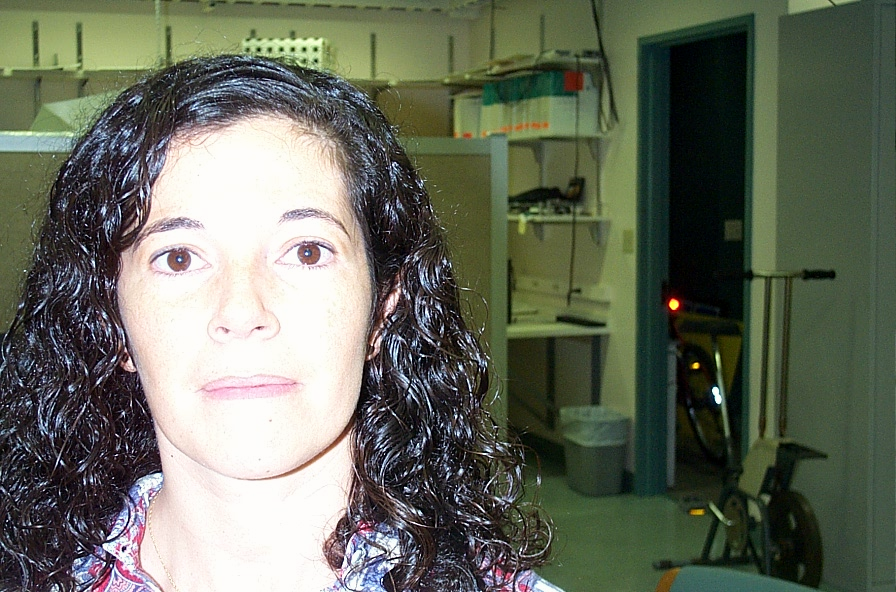
\includegraphics[width=0.95\textwidth]{img/fdResult1/input66.png}
  \caption{}
\end{subfigure}%
\begin{subfigure}{.33\textwidth}
  \centering
  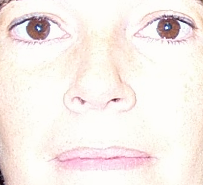
\includegraphics[width=0.6\textwidth]{img/fdResult1/output66.png}
  \caption{}
\end{subfigure}%
\end{subfigure}%
\begin{subfigure}{0.65\textwidth}
\begin{subfigure}{.33\textwidth}
  \centering
  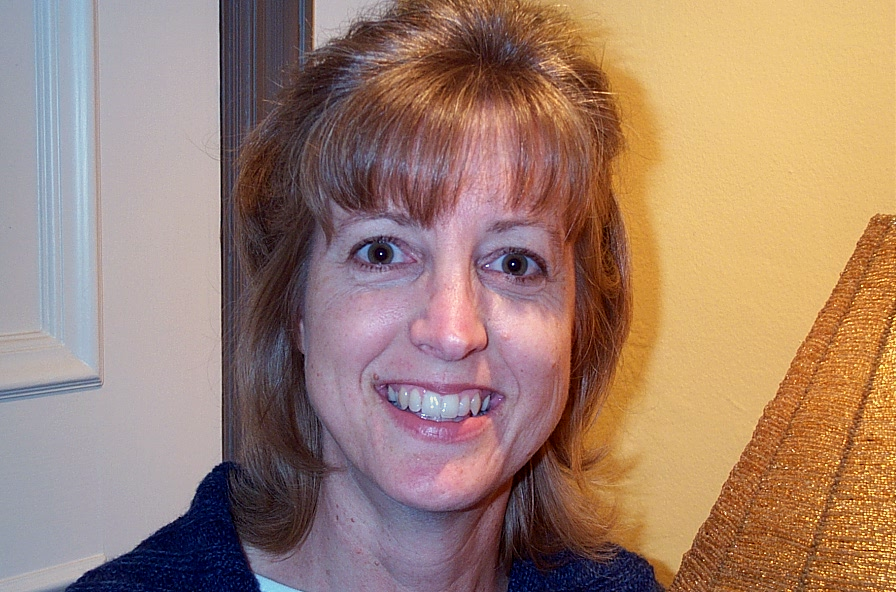
\includegraphics[width=0.95\textwidth]{img/fdResult1/input76.png}
  \caption{}
\end{subfigure}%
\begin{subfigure}{.33\textwidth}
  \centering
  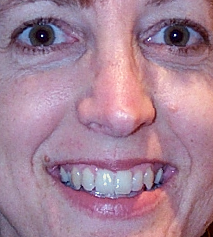
\includegraphics[width=0.6\textwidth]{img/fdResult1/output76.png}
  \caption{}
\end{subfigure}%
\end{subfigure}%

\caption{Results of the face detection phase depicting the algorithm's tolerance for varying environments \textit{(a-d)}, lightning conditions \textit{(e-h, m-p)}, poses \textit{(i-j)} and amount of skin color in the image \textit{(c-d, k-l)}.}


\label{fig:fdResults}
\end{figure}

\begin{figure}[H]
\centering

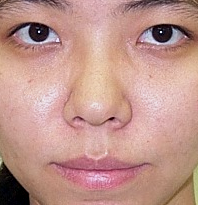
\includegraphics[width=0.09\textwidth]{img/fdResult1/output3.png}
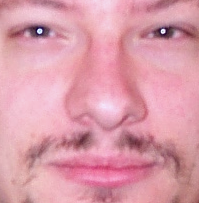
\includegraphics[width=0.09\textwidth]{img/fdResult1/output4.png}
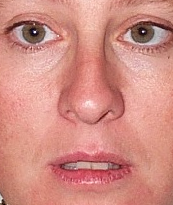
\includegraphics[width=0.09\textwidth]{img/fdResult1/output9.png}
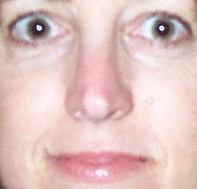
\includegraphics[width=0.09\textwidth]{img/fdResult1/output12.png}
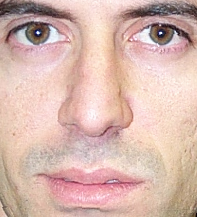
\includegraphics[width=0.09\textwidth]{img/fdResult1/output14.png}
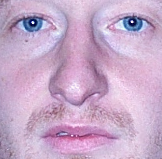
\includegraphics[width=0.09\textwidth]{img/fdResult1/output15.png}
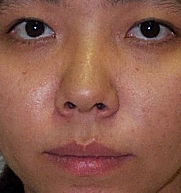
\includegraphics[width=0.09\textwidth]{img/fdResult1/output16.png}
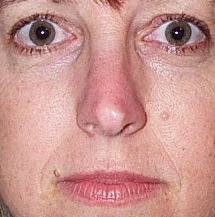
\includegraphics[width=0.09\textwidth]{img/fdResult1/output17.png}
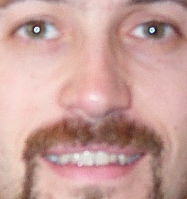
\includegraphics[width=0.09\textwidth]{img/fdResult1/output18.png}
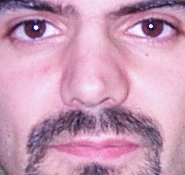
\includegraphics[width=0.09\textwidth]{img/fdResult1/output27.png}
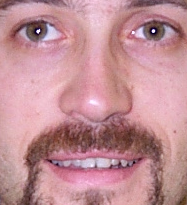
\includegraphics[width=0.09\textwidth]{img/fdResult1/output28.png}
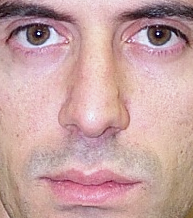
\includegraphics[width=0.09\textwidth]{img/fdResult1/output32.png}
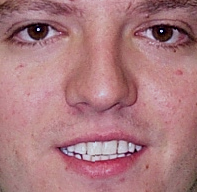
\includegraphics[width=0.09\textwidth]{img/fdResult1/output38.png}
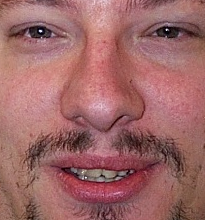
\includegraphics[width=0.09\textwidth]{img/fdResult1/output39.png}
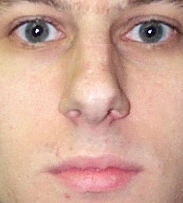
\includegraphics[width=0.09\textwidth]{img/fdResult1/output42.png}
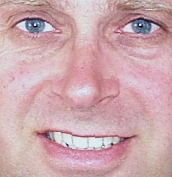
\includegraphics[width=0.09\textwidth]{img/fdResult1/output44.png}
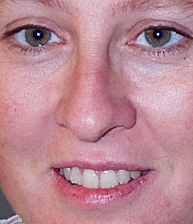
\includegraphics[width=0.09\textwidth]{img/fdResult1/output45.png}
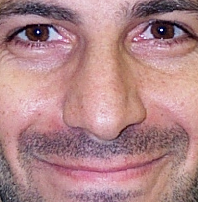
\includegraphics[width=0.09\textwidth]{img/fdResult1/output49.png}
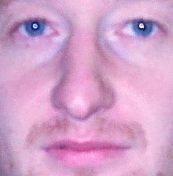
\includegraphics[width=0.09\textwidth]{img/fdResult1/output50.png}
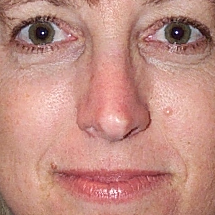
\includegraphics[width=0.09\textwidth]{img/fdResult1/output55.png}
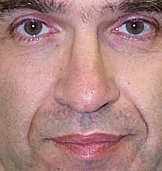
\includegraphics[width=0.09\textwidth]{img/fdResult1/output63.png}
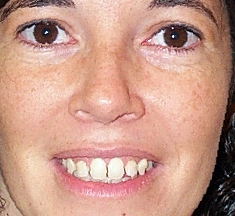
\includegraphics[width=0.09\textwidth]{img/fdResult1/output65.png}
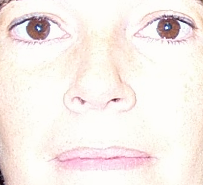
\includegraphics[width=0.09\textwidth]{img/fdResult1/output66.png}
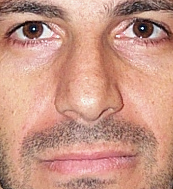
\includegraphics[width=0.09\textwidth]{img/fdResult1/output68.png}
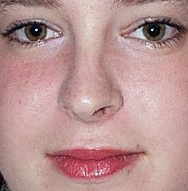
\includegraphics[width=0.09\textwidth]{img/fdResult1/output70.png}
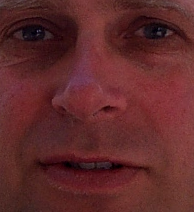
\includegraphics[width=0.09\textwidth]{img/fdResult1/output71.png}
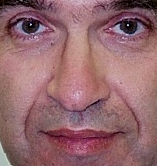
\includegraphics[width=0.09\textwidth]{img/fdResult1/output75.png}
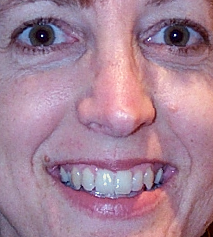
\includegraphics[width=0.09\textwidth]{img/fdResult1/output76.png}
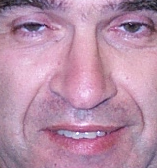
\includegraphics[width=0.09\textwidth]{img/fdResult1/output77.png}
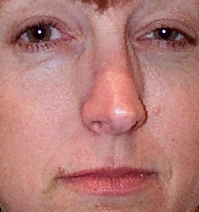
\includegraphics[width=0.09\textwidth]{img/fdResult1/output80.png}
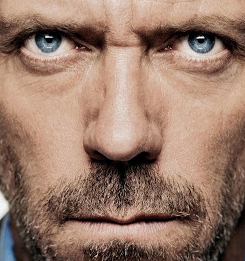
\includegraphics[width=0.09\textwidth]{img/fdResult2/output9.png}
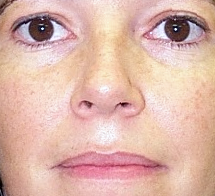
\includegraphics[width=0.09\textwidth]{img/fdResult1/output83.png}
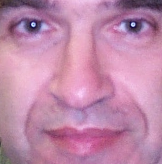
\includegraphics[width=0.09\textwidth]{img/fdResult1/output85.png}
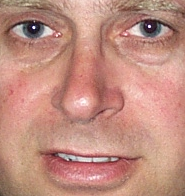
\includegraphics[width=0.09\textwidth]{img/fdResult1/output91.png}
\includegraphics[width=0.09\textwidth]{img/fdResult1/output92.png}
\includegraphics[width=0.09\textwidth]{img/fdResult1/output95.png}
\includegraphics[width=0.09\textwidth]{img/fdResult1/output96.png}
\includegraphics[width=0.09\textwidth]{img/fdResult1/output97.png}
\includegraphics[width=0.09\textwidth]{img/fdResult1/output98.png}
\includegraphics[width=0.09\textwidth]{img/fdResult2/output91.png}

\caption{Successful experimental results of face detection.}
\label{fig:faces}
\end{figure}

\begin{figure}[H]
\centering

\begin{subfigure}{.25\textwidth}
  \centering
  \includegraphics[width=0.95\textwidth]{img/fd3/fail1_input.jpg}
  \caption{}
\end{subfigure}%
\begin{subfigure}{.25\textwidth}
  \centering
  \includegraphics[width=0.95\textwidth]{img/fd3/fail1_faceImage.png}
  \caption{}
\end{subfigure}%
\begin{subfigure}{.25\textwidth}
  \centering
  \includegraphics[width=0.95\textwidth]{img/fd3/fail1_finalEyeMap.png}
  \caption{}
\end{subfigure}%
\begin{subfigure}{.25\textwidth}
  \centering
  \includegraphics[width=0.53\textwidth]{img/fd3/fail1_output.png}
  \caption{}
\end{subfigure}%

\caption{Resonera, Fail1}
\label{fig:fail1}
\end{figure}


\begin{figure}[H]
\centering

\begin{subfigure}{.25\textwidth}
  \centering
  \includegraphics[width=0.53\textwidth]{img/fd3/fail2_input.jpg}
  \caption{}
\end{subfigure}%
\begin{subfigure}{.25\textwidth}
  \centering
  \includegraphics[width=0.53\textwidth]{img/fd3/fail2_estimatedSkinMak.png}
  \caption{}
\end{subfigure}%
\begin{subfigure}{.25\textwidth}
  \centering
  \includegraphics[width=0.53\textwidth]{img/fd3/fail2_faceImage.png}
  \caption{}
\end{subfigure}%
\begin{subfigure}{.25\textwidth}
  \centering
  \includegraphics[width=0.23\textwidth]{img/fd3/fail2_output.png}
  \caption{}
\end{subfigure}%

\caption{Resonera, Fail2}
\label{fig:fail2}
\end{figure}




\begin{figure}[H]
\centering

\begin{subfigure}{.25\textwidth}
  \centering
  \includegraphics[width=0.53\textwidth]{img/fd3/fail3_input.jpg}
  \caption{}
\end{subfigure}%
\begin{subfigure}{.25\textwidth}
  \centering
  \includegraphics[width=0.53\textwidth]{img/fd3/fail3_faceBorder.png}
  \caption{}
\end{subfigure}%
\begin{subfigure}{.25\textwidth}
  \centering
  \includegraphics[width=0.53\textwidth]{img/fd3/fail3_eyeCandidates.png}
  \caption{}
\end{subfigure}%
% \begin{subfigure}{.15\textwidth}
%   \centering
%   \includegraphics[width=0.53\textwidth]{img/fd3/fail3_faceImage.png}
%   \caption{}
% \end{subfigure}%
% \begin{subfigure}{.15\textwidth}
%   \centering
%   \includegraphics[width=0.53\textwidth]{img/fd3/fail3_finalEyeMap.png}
%   \caption{}
% \end{subfigure}%
\begin{subfigure}{.25\textwidth}
  \centering
  \includegraphics[width=0.23\textwidth]{img/fd3/fail3_output.png}
  \caption{}
\end{subfigure}%

\caption{Resonera, Fail3}
\label{fig:fail3}
\end{figure}




\begin{figure}[H]
\centering

\begin{subfigure}{.25\textwidth}
  \centering
  \includegraphics[width=0.95\textwidth]{img/fd3/fail4_input.jpg}
  \caption{}
\end{subfigure}%
\begin{subfigure}{.25\textwidth}
  \centering
  \includegraphics[width=0.95\textwidth]{img/fd3/fail4_faceBorder.png}
  \caption{}
\end{subfigure}%
\begin{subfigure}{.25\textwidth}
  \centering
  \includegraphics[width=0.95\textwidth]{img/fd3/fail4_eyeCandidates.png}
  \caption{}
\end{subfigure}%
% \begin{subfigure}{.15\textwidth}
%   \centering
%   \includegraphics[width=0.95\textwidth]{img/fd3/fail4_faceImage.png}
%   \caption{}
% \end{subfigure}%
% \begin{subfigure}{.15\textwidth}
%   \centering
%   \includegraphics[width=0.95\textwidth]{img/fd3/fail4_finalEyeMap.png}
%   \caption{}
% \end{subfigure}%
\begin{subfigure}{.25\textwidth}
  \centering
  \includegraphics[width=0.53\textwidth]{img/fd3/fail4_output.png}
  \caption{}
\end{subfigure}%

\caption{Resonera, Fail4}
\label{fig:fail4}
\end{figure}








\subsection{Face recognition}
In this section the results obtained by the face recognition algorithm is  presented. The effects of performing face detection have been ignored in these results.

Table~\ref{tb:fr_results} show the results of applying the face recognition algorithm to the test data set.

\begin{center}
  \captionof{table}{Results of performing face recognition on the test data set.}
  \label{tb:fr_results}
    \begin{tabular}{ | l | l | l | l |}
    \hline
    Number of images & False positives & False negatives & Recognition Rate \\ \hline
    78 & 0 & 10 & 86\% \\ \hline
    \end{tabular}
\end{center}

Since the LPQ method used for face recognition is supposedly blur invariant, the effects of applying different types of blur to the input images where examined to verify this claim. Figure~\ref{fig:fr_result_plots_gauss} shows how the recognition rate is effected by applying Gaussian blur to the input images while Figure~\ref{fig:fr_result_plots_motion} shows the effect caused by a linear motion blur filter.

\begin{figure}[H]
\centering
\includegraphics[width=0.62\textwidth]{img/blur_test/gauss_plot.png}
\caption{Shows how applying Gaussian blur effects the recognition rate.}
\label{fig:fr_result_plots_gauss}
\end{figure}

\begin{figure}[H]
\centering
\includegraphics[width=0.62\textwidth]{img/blur_test/motion_plot.png}
\caption{Shows how applying linear motion blur effects the recognition rate.}
\label{fig:fr_result_plots_motion}
\end{figure}

Figure~\ref{fig:fr_result_plots_down} shows the result of decreasing the tone value and Figure~\ref{fig:fr_result_plots_up} shows the result of increasing the tone value.

\begin{figure}[H]
\centering
\includegraphics[width=0.62\textwidth]{img/blur_test/tone_down_plot.png}
\caption{Shows how reducing the tone value effects the recognition rate.}
\label{fig:fr_result_plots_down}
\end{figure}

\begin{figure}[H]
\centering
\includegraphics[width=0.62\textwidth]{img/blur_test/tone_up_plot.png}
\caption{Shows how increasing the tone value effects the recognition rate.}
\label{fig:fr_result_plots_up}
\end{figure}



\section{Discussion}
Write some discussion here :)

Ta upp dynamic thresholds etc etc...

Ta upp disk kernel

The face detection part of the algorithm can for example be improved by utilizing the facial expression normalization methods explored in  \cite{facialExpressions}.

FD

 FR


%----------------------------------------------------------------------------------------
% BIBLIOGRAPHY
%----------------------------------------------------------------------------------------

\bibliographystyle{unsrt}

\bibliography{references}


%----------------------------------------------------------------------------------------

\end{document}
